
%-----------------------------------------------------------------------------------------------------------------------------------------------%
%	The MIT License (MIT)
%
%	Copyright (c) 2019 Jan Küster
%
%	Permission is hereby granted, free of charge, to any person obtaining a copy
%	of this software and associated documentation files (the "Software"), to deal
%	in the Software without restriction, including without limitation the rights
%	to use, copy, modify, merge, publish, distribute, sublicense, and/or sell
%	copies of the Software, and to permit persons to whom the Software is
%	furnished to do so, subject to the following conditions:
%	
%	THE SOFTWARE IS PROVIDED "AS IS", WITHOUT WARRANTY OF ANY KIND, EXPRESS OR
%	IMPLIED, INCLUDING BUT NOT LIMITED TO THE WARRANTIES OF MERCHANTABILITY,
%	FITNESS FOR A PARTICULAR PURPOSE AND NONINFRINGEMENT. IN NO EVENT SHALL THE
%	AUTHORS OR COPYRIGHT HOLDERS BE LIABLE FOR ANY CLAIM, DAMAGES OR OTHER
%	LIABILITY, WHETHER IN AN ACTION OF CONTRACT, TORT OR OTHERWISE, ARISING FROM,
%	OUT OF OR IN CONNECTION WITH THE SOFTWARE OR THE USE OR OTHER DEALINGS IN
%	THE SOFTWARE.
%	
%
%-----------------------------------------------------------------------------------------------------------------------------------------------%


%============================================================================%
%
%	DOCUMENT DEFINITION
%
%============================================================================%

%we use article class because we want to fully customize the page and don't use a cv template
\documentclass[10pt,A4]{article}	


%----------------------------------------------------------------------------------------
%	ENCODING
%----------------------------------------------------------------------------------------

% we use utf8 since we want to build from any machine
\usepackage[utf8]{inputenc}		

%----------------------------------------------------------------------------------------
%	LOGIC
%----------------------------------------------------------------------------------------

% provides \isempty test
\usepackage{xstring, xifthen}

%----------------------------------------------------------------------------------------
%	FONT BASICS
%----------------------------------------------------------------------------------------

% some tex-live fonts - choose your own

%\usepackage[defaultsans]{droidsans}
%\usepackage[default]{comfortaa}
%\usepackage{cmbright}
\usepackage[default]{raleway}
%\usepackage{fetamont}
%\usepackage[default]{gillius}
%\usepackage[light,math]{iwona}
%\usepackage[thin]{roboto} 

% set font default
\renewcommand*\familydefault{\sfdefault} 	
\usepackage[T1]{fontenc}

% more font size definitions
\usepackage{moresize}

%----------------------------------------------------------------------------------------
%	FONT AWESOME ICONS
%---------------------------------------------------------------------------------------- 

% include the fontawesome icon set
\usepackage{fontawesome}

% use to vertically center content
% credits to: http://tex.stackexchange.com/questions/7219/how-to-vertically-center-two-images-next-to-each-other
\newcommand{\vcenteredinclude}[1]{\begingroup
\setbox0=\hbox{\includegraphics{#1}}%
\parbox{\wd0}{\box0}\endgroup}

% use to vertically center content
% credits to: http://tex.stackexchange.com/questions/7219/how-to-vertically-center-two-images-next-to-each-other
\newcommand*{\vcenteredhbox}[1]{\begingroup
\setbox0=\hbox{#1}\parbox{\wd0}{\box0}\endgroup}

% icon shortcut
\newcommand{\icon}[3] { 							
	\makebox(#2, #2){\textcolor{maincol}{\csname fa#1\endcsname}}
}	

% icon with text shortcut
\newcommand{\icontext}[4]{ 						
	\vcenteredhbox{\icon{#1}{#2}{#3}}  \hspace{2pt}  \parbox{0.9\mpwidth}{\textcolor{#4}{#3}}
}

% icon with website url
\newcommand{\iconhref}[5]{ 						
    \vcenteredhbox{\icon{#1}{#2}{#5}}  \hspace{2pt} \href{#4}{\textcolor{#5}{#3}}
}

% icon with email link
\newcommand{\iconemail}[5]{ 						
    \vcenteredhbox{\icon{#1}{#2}{#5}}  \hspace{2pt} \href{mailto:#4}{\textcolor{#5}{#3}}
}

%----------------------------------------------------------------------------------------
%	PAGE LAYOUT  DEFINITIONS
%----------------------------------------------------------------------------------------

% page outer frames (debug-only)
% \usepackage{showframe}		

% we use paracol to display breakable two columns
\usepackage{paracol}

% define page styles using geometry
\usepackage[a4paper]{geometry}

% remove all possible margins
\geometry{top=1cm, bottom=1cm, left=1cm, right=1cm}

\usepackage{fancyhdr}
\pagestyle{empty}

% space between header and content
% \setlength{\headheight}{0pt}

% indentation is zero
\setlength{\parindent}{0mm}

%----------------------------------------------------------------------------------------
%	TABLE /ARRAY DEFINITIONS
%---------------------------------------------------------------------------------------- 

% extended aligning of tabular cells
\usepackage{array}

% custom column right-align with fixed width
% use like p{size} but via x{size}
\newcolumntype{x}[1]{%
>{\raggedleft\hspace{0pt}}p{#1}}%


%----------------------------------------------------------------------------------------
%	GRAPHICS DEFINITIONS
%---------------------------------------------------------------------------------------- 

%for header image
\usepackage{graphicx}

% use this for floating figures
 \usepackage{wrapfig}
 \usepackage{float}
 \floatstyle{boxed} 
 \restylefloat{figure}

%for drawing graphics		
\usepackage{tikz}				
\usetikzlibrary{shapes, backgrounds,mindmap, trees}

%----------------------------------------------------------------------------------------
%	Color DEFINITIONS
%---------------------------------------------------------------------------------------- 
\usepackage{transparent}
\usepackage{color}

% primary color
\definecolor{maincol}{RGB}{ 45, 50, 90 }

% accent color, secondary
% \definecolor{accentcol}{RGB}{ 250, 150, 10 }

% dark color
\definecolor{darkcol}{RGB}{ 70, 70, 70 }

% light color
\definecolor{lightcol}{RGB}{245,245,245}


% Package for links, must be the last package used
\usepackage[hidelinks]{hyperref}

% returns minipage width minus two times \fboxsep
% to keep padding included in width calculations
% can also be used for other boxes / environments
\newcommand{\mpwidth}{\linewidth-\fboxsep-\fboxsep}
	


%============================================================================%
%
%	CV COMMANDS
%
%============================================================================%

%----------------------------------------------------------------------------------------
%	 CV LIST
%----------------------------------------------------------------------------------------

% renders a standard latex list but abstracts away the environment definition (begin/end)
\newcommand{\cvlist}[1] {
	\begin{itemize}{#1}\end{itemize}
}

%----------------------------------------------------------------------------------------
%	 CV TEXT
%----------------------------------------------------------------------------------------

% base class to wrap any text based stuff here. Renders like a paragraph.
% Allows complex commands to be passed, too.
% param 1: *any
\newcommand{\cvtext}[1] {
	\begin{tabular*}{1\mpwidth}{p{0.98\mpwidth}}
		\parbox{1\mpwidth}{#1}
	\end{tabular*}
}

%----------------------------------------------------------------------------------------
%	CV SECTION
%----------------------------------------------------------------------------------------

% Renders a a CV section headline with a nice underline in main color.
% param 1: section title
\newcommand{\cvsection}[1] {
	\vspace{14pt}
	\cvtext{
		\textbf{\LARGE{\textcolor{darkcol}{\uppercase{#1}}}}\\[-4pt]
		\textcolor{maincol}{ \rule{0.1\textwidth}{2pt} } \\
	}
}

%----------------------------------------------------------------------------------------
%	META SKILL
%----------------------------------------------------------------------------------------

% Renders a progress-bar to indicate a certain skill in percent.
% param 1: name of the skill / tech / etc.
% param 2: level (for example in years)
% param 3: percent, values range from 0 to 1
\newcommand{\cvskill}[3] {
	\begin{tabular*}{1\mpwidth}{p{0.72\mpwidth}  r}
 		\textcolor{black}{\textbf{#1}} & \textcolor{maincol}{#2}\\
	\end{tabular*}%
	
	\hspace{4pt}
	\begin{tikzpicture}[scale=1,rounded corners=2pt,very thin]
		\fill [lightcol] (0,0) rectangle (1\mpwidth, 0.15);
		\fill [maincol] (0,0) rectangle (#3\mpwidth, 0.15);
  	\end{tikzpicture}%
}


%----------------------------------------------------------------------------------------
%	 CV EVENT
%----------------------------------------------------------------------------------------

% Renders a table and a paragraph (cvtext) wrapped in a parbox (to ensure minimum content
% is glued together when a pagebreak appears).
% Additional Information can be passed in text or list form (or other environments).
% the work you did
% param 1: time-frame i.e. Sep 14 - Jan 15 etc.
% param 2:	 event name (job position etc.)
% param 3: Customer, Employer, Industry
% param 4: Short description
% param 5: work done (optional)
% param 6: technologies include (optional)
% param 7: achievements (optional)
\newcommand{\cvevent}[7] {
	
	% we wrap this part in a parbox, so title and description are not separated on a pagebreak
	% if you need more control on page breaks, remove the parbox
	\parbox{\mpwidth}{
		\begin{tabular*}{1\mpwidth}{p{0.72\mpwidth}  r}
	 		\textcolor{black}{\textbf{#2}} & \colorbox{maincol}{\makebox[0.25\mpwidth]{\textcolor{white}{#1}}} \\
			\textcolor{maincol}{\textbf{#3}} & \\
		\end{tabular*}\\[4pt]
	
		\ifthenelse{\isempty{#4}}{}{
			\cvtext{#4}\\
		}
	}

	\ifthenelse{\isempty{#5}}{}{
		\vspace{4pt}
		{#5}
	}
	\vspace{4pt}
}

\newcommand{\cveventOne}[7] {
	
	% we wrap this part in a parbox, so title and description are not separated on a pagebreak
	% if you need more control on page breaks, remove the parbox
	\parbox{\mpwidth}{
		\begin{tabular*}{1\mpwidth}{p{0.72\mpwidth}  r}
        
			\textcolor{maincol}{\textbf{#3}}  &
			 \colorbox{maincol}{\makebox[0.25\mpwidth]{\textcolor{white}{#1}}} \\
		\end{tabular*}\\[4pt]
	
		\ifthenelse{\isempty{#4}}{}{
			\cvtext{#4}\\
		}
	}

	\ifthenelse{\isempty{#5}}{}{
		\vspace{4pt}
		{#5}
	}
	\vspace{4pt}
}

\newcommand{\cveventp}[7] {
	
	% we wrap this part in a parbox, so title and description are not separated on a pagebreak
	% if you need more control on page breaks, remove the parbox
	\parbox{\mpwidth}{
		\begin{tabular*}{1\mpwidth}{p{0.72\mpwidth}  r}
	 		\textcolor{black}{\textbf{#2}} & \colorbox{maincol}{\makebox[0.25\mpwidth]{\textcolor{white}{#1}}} \\
			\textcolor{maincol}{\textbf{#3}} &   \\
		\end{tabular*}\\[4pt]
	
	 % 	\begin{wrapfigure}[\textwidth]{r}{\textwidth}
	 %   	    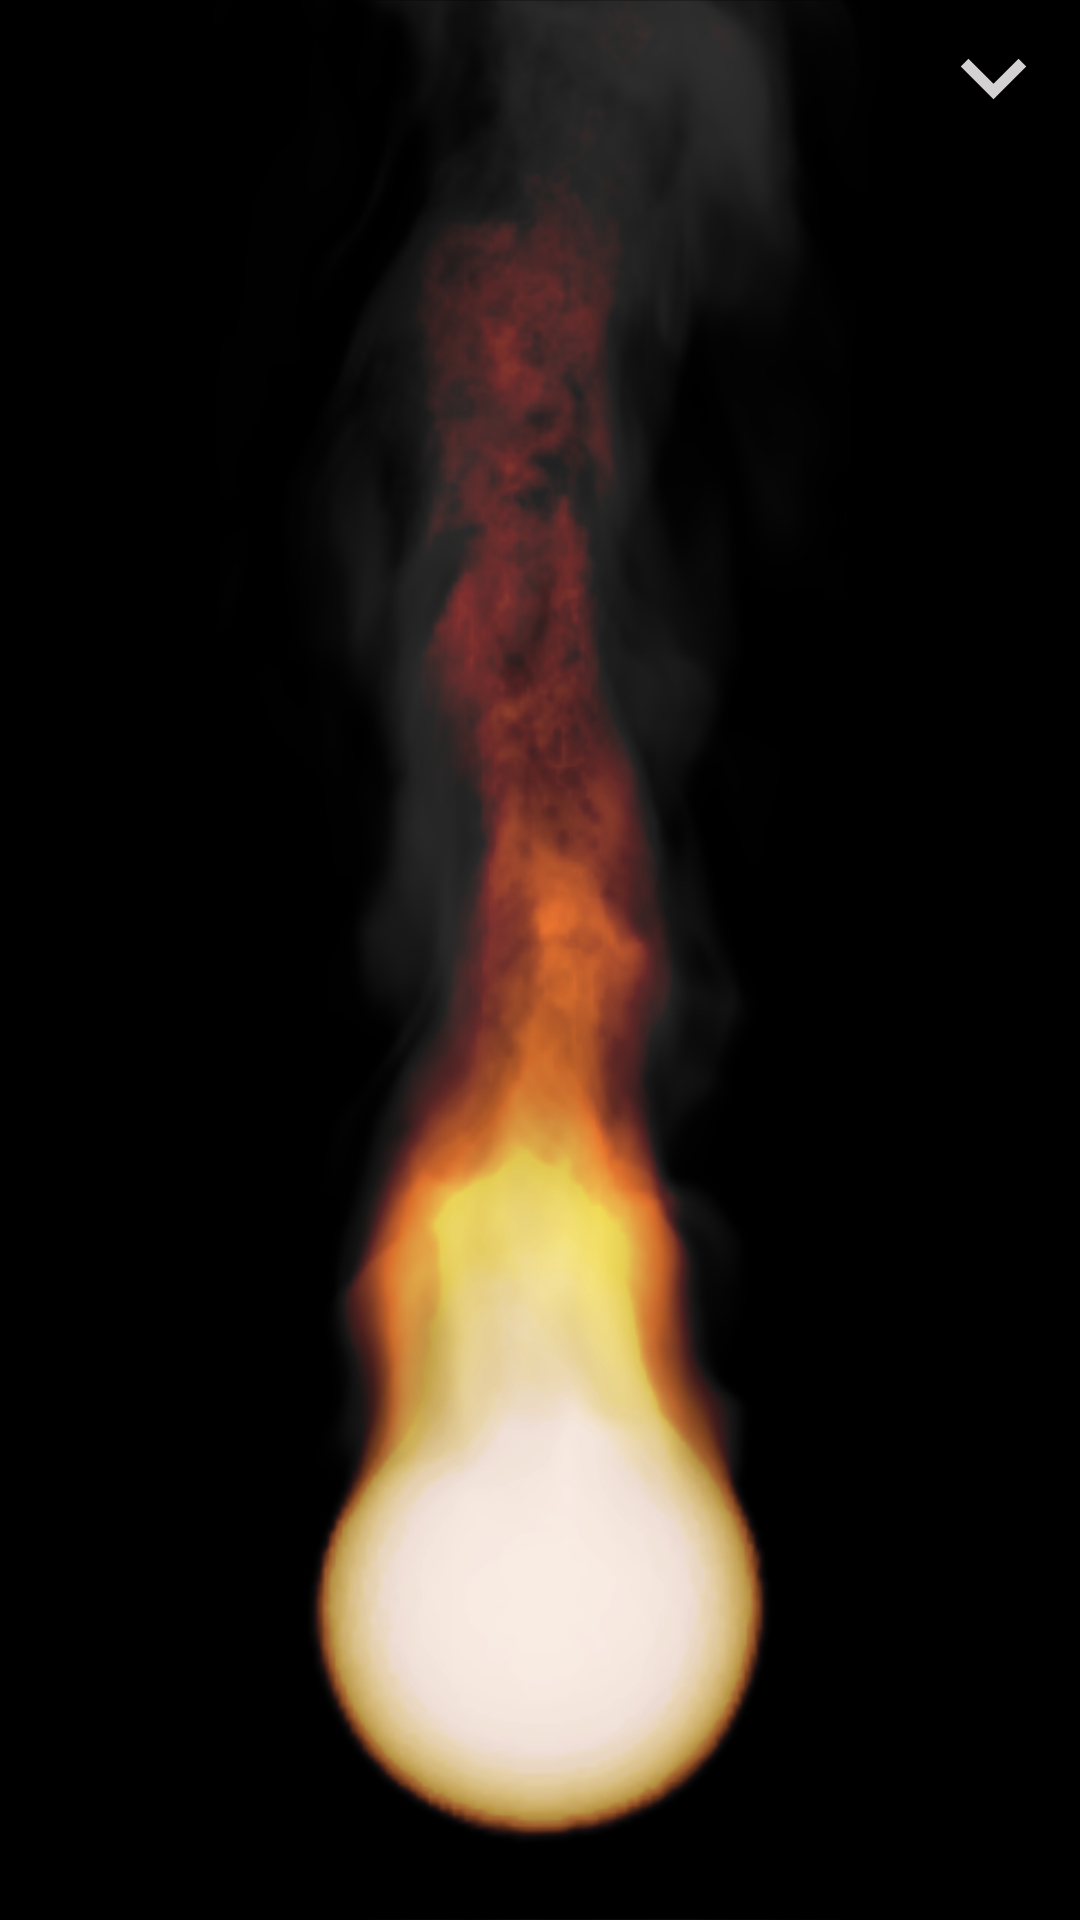
\includegraphics[width=100px]{bilder/eld.jpg}
	 %   \end{wrapfigure}
	    
		\ifthenelse{\isempty{#4}}{}{
			\cvtext{#4}\\
			
		}
	}

	\ifthenelse{\isempty{#5}}{}{
		\vspace{4pt}
		{#5}
	}
	\vspace{4pt}
}

%----------------------------------------------------------------------------------------
%	 CV META EVENT
%----------------------------------------------------------------------------------------

% Renders a CV event on the sidebar
% param 1: title
% param 2: subtitle (optional)
% param 3: customer, employer, etc,. (optional)
% param 4: info text (optional)
\newcommand{\cvmetaevent}[4] {
	\textcolor{maincol} {\cvtext{\textbf{\begin{flushleft}#1\end{flushleft}}}}

	\ifthenelse{\isempty{#2}}{}{
	\textcolor{darkcol} {\cvtext{\textbf{#2}} }
	}

	\ifthenelse{\isempty{#3}}{}{
		\cvtext{{ \textcolor{darkcol} {#3} }}\\
	}

	\cvtext{#4}\\[14pt]
}

%---------------------------------------------------------------------------------------
%	QR CODE
%----------------------------------------------------------------------------------------

% Renders a qrcode image (centered, relative to the parentwidth)
% param 1: percent width, from 0 to 1
\newcommand{\cvqrcode}[1] {
	\begin{center}
		\includegraphics[width={#1}\mpwidth]{qrcode}
	\end{center}
}

%=+=+=+=+=+=+=+=+=+=+=+=+=+=+=+=+=+=+=+=+=+=+=+=+=+=+=+=+=+=+=+=+=+=+=+=+=+=+=+=+
%,,,,,,,,,,,,,,,,,,,,,,,,,,,,,,,,,,,,,,,,,,,,,,,,,,,,,,,,,,,,,,,,,,,,,,,,,,,,,,,,
                       % EDIT AFTER THIS POINT
%''''''''''''''''''''''''''''''''''''''''''''''''''''''''''''''''''''''''''''''''
%=+=+=+=+=+=+=+=+=+=+=+=+=+=+=+=+=+=+=+=+=+=+=+=+=+=+=+=+=+=+=+=+=+=+=+=+=+=+=+=+


%============================================================================%
%
%
%
%	DOCUMENT CONTENT
%
%
%
%============================================================================%
\begin{document}
\columnratio{0.31}
\setlength{\columnsep}{2.2em}
\setlength{\columnseprule}{4pt}
\colseprulecolor{lightcol}
\begin{paracol}{2}
\begin{leftcolumn}
%---------------------------------------------------------------------------------------
%	META IMAGE
%----------------------------------------------------------------------------------------
%\includegraphics[width=\linewidth]{untitled.jpg}	%trimming relative to image size


\vfill\null
\cvsection{Kontakt}
	
\iconemail{EnvelopeSquare}{14}{contact@anton-forsberg.com}{contact@anton-forsberg.com}{black}\\[6pt]
\icontext{Globe}{14}{\href{https://anton-forsberg.com}{https://anton-forsberg.com}}{black}\\[6pt]
\icontext{Github}{14}{\href{https://github.com/antfor}{https://github.com/antfor}}{black}\\[6pt]
\icontext{Phone}{14}{072 448 23 20}{black}\\[6pt]
\icontext{Home}{14}{Döbelnsgatan 6a \newline 752 37 Uppsala  }{black}\\[6pt]
\icontext{User}{14}{19980112}{black}\\[6pt]
%\icontext{Linkedin}{14}{\href{https://www.linkedin.com/in/yourid/}{yourid}}{black}\\[6pt]

\vfill\null
%\cvqrcode{0.7}

%---------------------------------------------------------------------------------------
%	META SKILLS
%----------------------------------------------------------------------------------------
\cvsection{Kompetens}

%\cvskill{Skill_Name} {Years of experience} {percentage of bar fill} \\[-2pt]
\cvskill{JavaScript/TypeScript} {} {1} \\[-2pt]

\cvskill{Java} {} {1} \\[-2pt]

\cvskill{Python} {} {1} \\[-2pt]

\cvskill{C++} {} {1} \\[-2pt]

\cvskill{C\#} {} {1} \\[-2pt]

\cvskill{haskell} {} {1} \\[-2pt]

\cvskill{erlang} {} {1} \\[-2pt]

\cvskill{opengl} {} {1} \\[-2pt]

\cvskill{Android and Xamarin app utväckling} {} {1} \\[-2pt]

\cvskill{ARM, RISC-V} {} {1} \\[-2pt]

\cvskill{linux} {} {1} \\[-2pt]




%\vfill\null
%\cvqrcode{0.7}

%---------------------------------------------------------------------------------------
%	ACHIEVEMENTS
%----------------------------------------------------------------------------------------
\newpage

\end{leftcolumn}
\begin{rightcolumn}
%---------------------------------------------------------------------------------------
%	TITLE  HEADER
%----------------------------------------------------------------------------------------
\fcolorbox{white}{darkcol}{\begin{minipage}[c][1.5cm][c]{1\mpwidth}
	\begin {center}
		\HUGE{ \textbf{ \textcolor{white}{ \uppercase{ Anton Forsberg} } } } \\[-24pt]
		%\textcolor{white}{ \rule{0.1\textwidth}{1.25pt} } \\[4pt]
		%\large{ \textcolor{white} { } }
	\end {center}
\end{minipage}} \\[14pt]
\vspace{-12pt}
% intro
\cvsection{Sammanfattning}
%Jag tycker även om den social aspekten av programmering, via ett nära samarbete med andra utvecklare. 
\cvtext{Jag är en programmeringsintresserad civilingenjör som har erfarenhet av olika programspråk och designprinciper.  Jag gillar att lära mig nya språk och arbetssätt och den senaste tiden har jag utvecklat min hemsida för att lära mig webutveckling.}
\vspace{4pt}
%---------------------------------------------------------------------------------------
%	EDUCATION
%----------------------------------------------------------------------------------------
%\vfill\null
\cvsection{Utbildning}

\begin{wrapfigure}[2]{R}{0.08\textwidth}
   \vspace{-60pt}
    \begin{center}
    
\includegraphics[width=0.12\textwidth]{bilder/chalmers.png}
     \end{center}
\end{wrapfigure}


\cvevent
	{\textbf{2017 - 2023}}
	{Civilingenjörsexamen och masterexamen}
	{Chalmers tekniska högskola}
	{
    Examen från Chalmers med inriktning på informations- teknik och datavetenskap, har givit mig breda kunskaper inom programmering.
    \newline
    \textbf{Masteruppsats:}
    \newline
    Optimera hastigheten av  Convolutional Neural Networks (CNN) med nya vektor instruktioner från ARM och RISC-V.
    \newline
    \textbf{Thesis:}
    \newline
    \url{http://hdl.handle.net/20.500.12380/307458}
    \newline
    \textbf{Repository:}
	\newline
	\url{https://github.com/antfor/Masters-NNPACK}
    \newline
	\url{https://github.com/antfor/Masters-darknet}
    }
	{}
	
\vfill\null
\vspace{4pt}
%---------------------------------------------------------------------------------------
%	Project
%----------------------------------------------------------------------------------------

\cvsection{Projekt}

\begin{wrapfigure}[2]{R}{0.08\textwidth}
   \vspace{-70pt}
    \begin{center}
    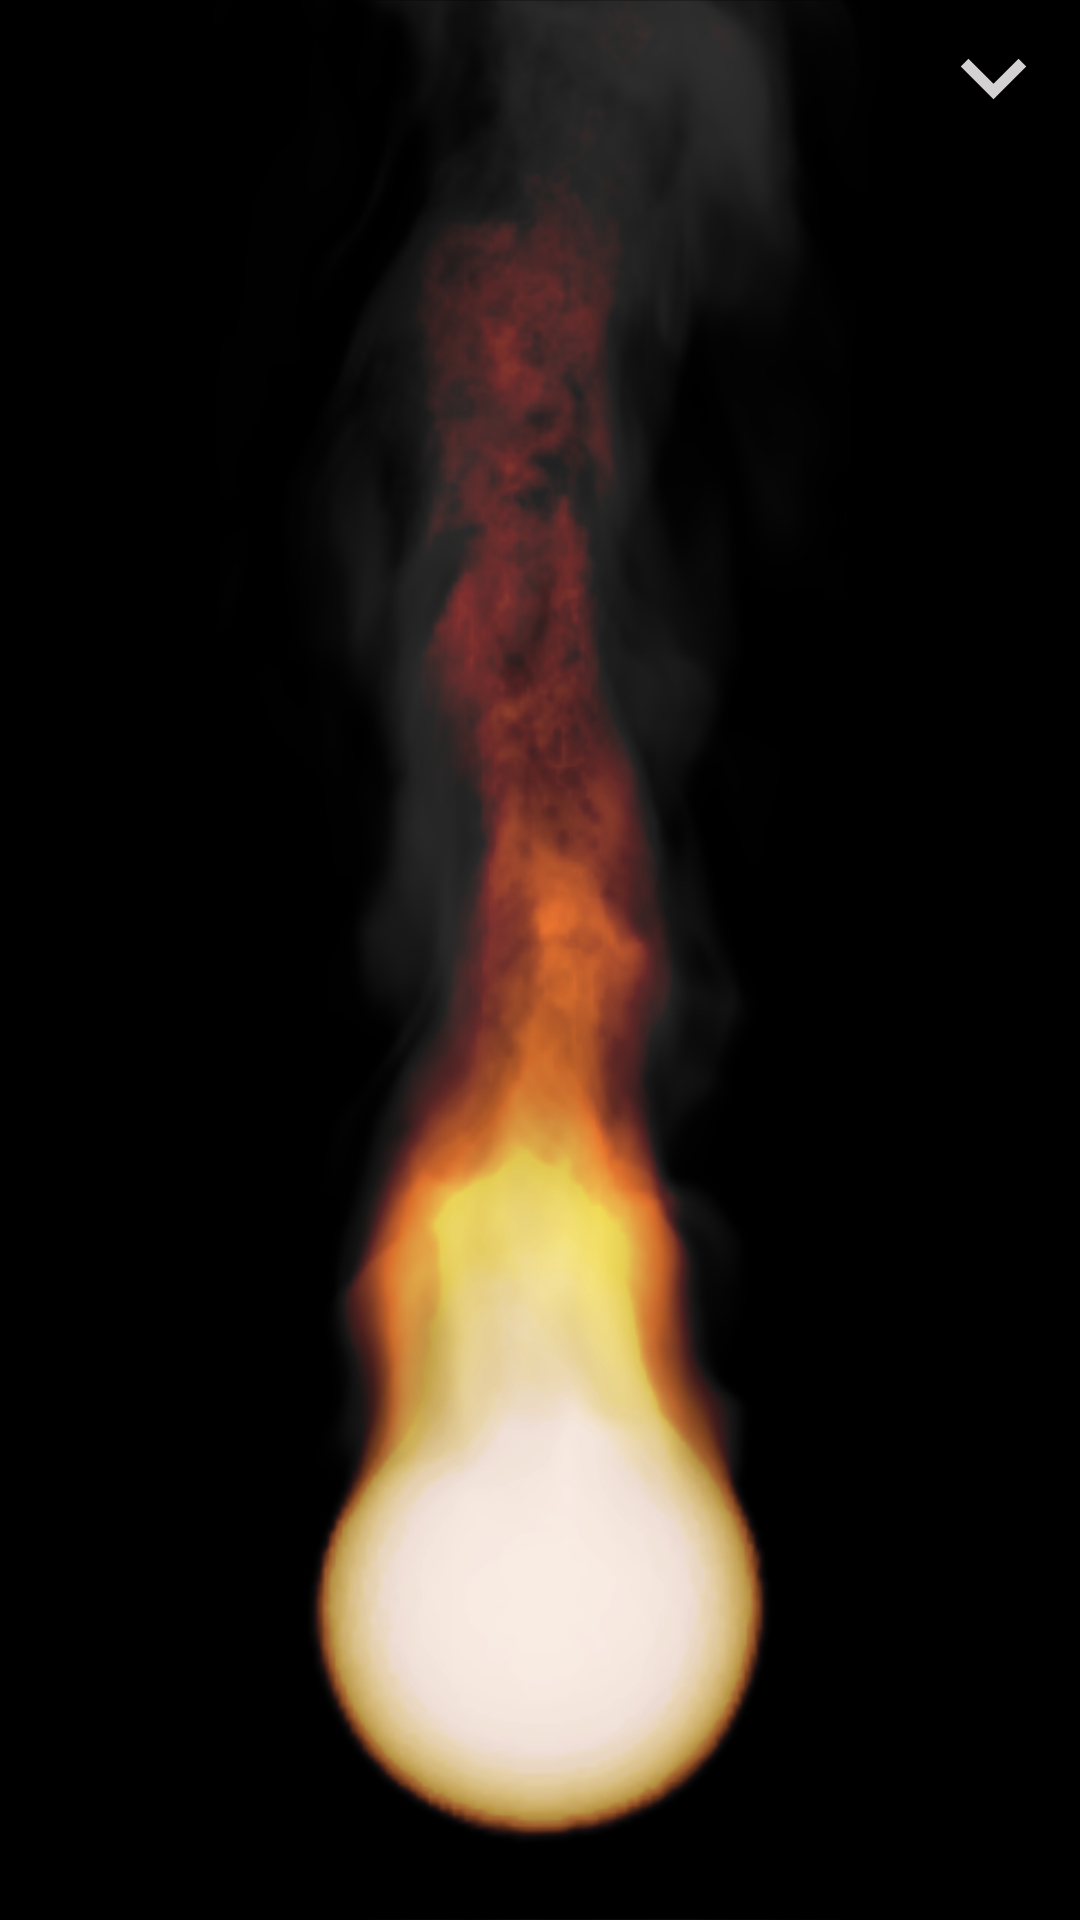
\includegraphics[width=0.12\textwidth]{bilder/eld.jpg}
     \end{center}
    \vspace{10pt}
    \begin{center}
    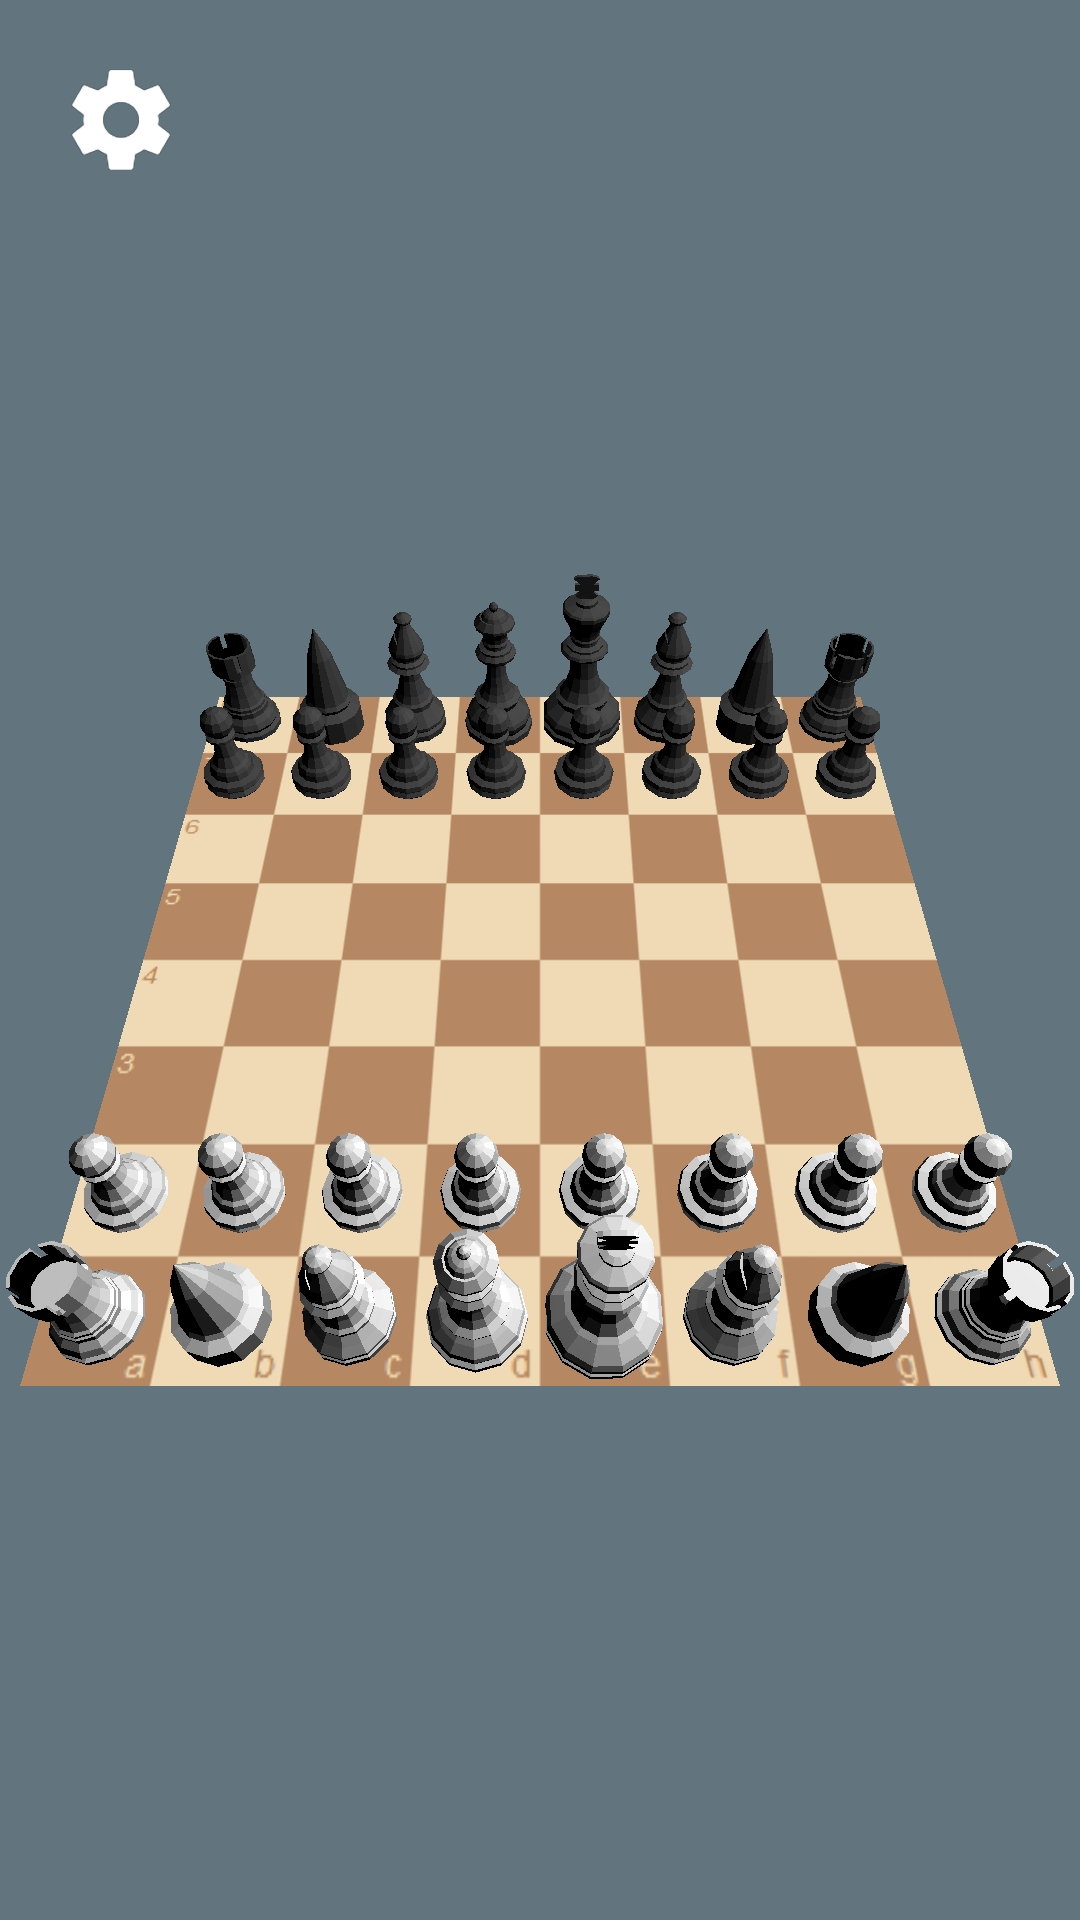
\includegraphics[width=0.12\textwidth]{bilder/schack.jpg}
    \end{center}
\end{wrapfigure}

\cvevent
	{\textbf{Jan - Maj 2020}}
	{Kandidatarbetet}
	{Physically-Based Animation of \newline Fire for Android}
	{
	Under kandidatarbetet samarbetade jag med fem personer där vi höll oss till scrum som    arbetssätt. \newline
    Utöver programmeringsarbetet bidrog jag med initiativ och att driva projektet framåt.\newline 
    Som helhet ledde allt detta till ett mycket lyckat resulta. 
    \newline
    \textbf{Thesis:}
    \newline
    \url{http://hdl.handle.net/20.500.12380/307458}
    \newline
    \textbf{Repository:}
    \newline
    \url{https://github.com/antfor/Bachelors}
    }
	{}
\vfill\null
\vspace{8pt}
\cvevent
	{\textbf{Maj - Dec 2017}}
	{Fritid}
	{Spelmotor och schackspel i 3D grafik på Android}
	{På min fritid har jag exempelvis jobbat med att lära mig att programmera för grafikkortet (openGL) och app utveckling.
	\newline
	Bland annat har jag skapat en spelmotor som jag använt för att göra en 3D schack app.
	\newline
	\textbf{Repository:}
	\newline
	\url{https://github.com/antfor/Chess-and-AndroidGameEngine}
	%\newline
    }
	{}
%\vfill\null
%---------------------------------------------------------------------------------------
%	PUBLICATION
%----------------------------------------------------------------------------------------
%\vspace{-0.5cm}
\vfill\null

% \cvsection{Erfarenheter}

% \cveventOne
% 	{\textbf{pågående}}
% 	{}
% 	{Generella kunskaper}
% 	{Har en relativt bred erfarenhet av olika programspråk och designprinciper i olika programmeringsparadigm. Därav kan jag ganska snabbt plocka upp nya språk/principer/verktyg om det behövs för att lösa \newline arbetsuppgifter. \newline Har på senaste tiden jobbat på min hemsida för att lära mig web utväckling.}
% 	{}
% \vfill\null

%\cveventOne
%	{\textbf{2016 - pågående}}
%	{}
%	{Programering}
%	{Jag har hållit på med olika former av programmering i ungefär 6-7 år.}
%	{ }
%\vfill\null

%---------------------------------------------------------------------------------------
%	SKILLS
%----------------------------------------------------------------------------------------

%---------------------------------------------------------------------------------------
%	PERSONAL DETAILS
%----------------------------------------------------------------------------------------
%\vfill\null
%\cvsection{EXTRACURRICULAR}
%\vspace{-0.3cm}
%\begin{itemize}
%  \item Put all the points that are not covered in \textbf{above sections}.
%  \item Put all the points that are \textbf{not covered} in above sections.
%  \item Put all the \textbf{points} that are not covered in above sections.
%  \item \textbf{Put all the points} that are not covered in above sections.
%\end{itemize}
%\vfill\null


% hotfixes to create fake-space to ensure the whole height is used
\vfill
\vfill
\vfill
\end{rightcolumn}
\end{paracol}
\end{document}